\documentclass[11pt,letterpaper]{article}

% MallorcaPlant — NeurIPS Datasets & Benchmarks layout (mirrors GeoPlant structure).
% Compile:
%   export TEXMFVAR="$(pwd)/.texmf-var" TEXMFCACHE="$(pwd)/.texmf-var"
%   pdflatex main && pdflatex main

\usepackage[utf8]{inputenc}
\usepackage[T1]{fontenc}
\usepackage[margin=1in]{geometry}
\usepackage{natbib}
\usepackage{hyperref}
\usepackage{url}
\usepackage{booktabs}
\usepackage{amsmath}
\usepackage{amssymb}
\usepackage{graphicx}

\hypersetup{colorlinks=true,linkcolor=blue,citecolor=blue,urlcolor=blue}
\bibliographystyle{apalike}

\title{MallorcaPlant: A Precision Multi-Source Dataset\\for Plant Species Distribution Modeling}

\author{%
  Iv\'an Cort\'es-Fern\'andez\thanks{Product Lead; affiliations to be confirmed.}\\
  University of the Balearic Islands (UIB)
  \and
  Pablo Ubilla Pavez\\
  INRIA Montpellier
  \and
  Diego Marcos\\
  INRIA / Universit\'e de Montpellier
  % TODO: confirm final author list with Diego before freeze
}

\date{}

\begin{document}

\maketitle

\begin{abstract}
Over roughly \textbf{40 years} of field campaigns on Mallorca (Balearic Islands, Spain), local botanists have generated a large corpus of largely \textbf{unpublished} floristic surveys and plot inventories, amounting to hundreds of thousands of occurrence records (preliminary assembly: \textbf{351\,980} presence records).
We release \textbf{MallorcaPlant}, a multi-source terrestrial vascular-plant dataset that makes this effort usable for species distribution modeling (SDM).
Beyond raw counts, the resource encodes observation semantics that aggregators usually hide: complete versus incomplete atlas Presence--Absence (\textbf{PAC}/\textbf{PAU}), expert-validated Presence-Only from a regional platform (\textbf{POV}), and unvalidated Presence-Only from GBIF (\textbf{POU}).
Validated PO records were curated by local experts; taxonomic strings were matched and cleaned \textbf{one by one} against the GBIF backbone (largely inheriting Plants of the World Online), including names absent from or rejected by GBIF because of ongoing taxonomic change or undescribed entities under local monitoring.
Environmental predictors include a dynamically downscaled 1\,km Balearic climate stack \citep{bahuet2026}, land cover, topography, taxonomic covariates, and satellite embeddings that deliberately exclude GBIF-pretrained foundations such as AlphaEarth.
We provide a transfer benchmark---train on PAU/POV/POU (and mixes), evaluate mean per-species ROC-AUC on PAC---with weak and strong baselines.
Preliminary mixes reach mean PAC AUC around $0.76$ when validated POV is included; figures remain provisional pending full-island coverage and spatial block cross-validation.
\end{abstract}

\noindent\textit{NeurIPS Track on Datasets and Benchmarks --- draft formatting.}


% ---------------------------------------------------------------------------
\section{Introduction}
\label{sec:intro}

Global change transforms ecosystems at fine scales that are hard to monitor exhaustively \citep{geoplant2024}.
Deep SDMs map many taxa jointly from high-resolution predictors \citep{geoplant2024}, but they inherit messy biodiversity data: structured inventories remain scarce, while GBIF and similar aggregators supply millions of Presence-Only (PO) points that lack true absences and concentrate near observers \citep{insects16080769,phillips2009sample}.

A less discussed problem is \textbf{hidden information} inside those streams.
Atlas-style Presence--Absence (PA) surveys are frequently ingested and redistributed as if they were PO points: the survey protocol, grid geometry, and implied absences are stripped, so models treat exhaustive inventories like opportunistic sightings.
PA tables also often lack collection dates (or carry only campaign-level metadata), which makes it extremely difficult to reconstruct sampling effort over time or to estimate sampling coverage for detectability and integrated models \citep{isaac2020data,fletcher2019practical}.
Without author contact and local metadata, completeness of a grid cell and validation status of a GPS point remain invisible.

MallorcaPlant addresses that gap with island-scale precision.
About four decades of own floristic work, local plot inventories, a regional expert-validated occurrence platform, and GBIF downloads coexist on one island.
Direct access to primary survey authors lets us recover four observation classes---PAC, PAU, POV, and POU (Section~\ref{sec:dataset})---and to audit every taxonomic string manually.
The GBIF taxonomic backbone (drawing heavily on Plants of the World Online, POWO) is used as a shared key, but local usage often diverges from accepted GBIF names; those cases were resolved case by case rather than dropped silently.

\paragraph{Contributions.}
(1)~A multi-source plant occurrence dataset with explicit PAC/PAU/POV/POU labels, rooted in decades of local surveys and unpublished inventories.
(2)~Expert-validated PO plus one-by-one taxonomic cleaning by local botanists, including taxa not accepted or not listed in GBIF.
(3)~Multimodal predictors: fine Balearic climate \citep{bahuet2026}, land use, topography, taxonomic features, and non--GBIF-pretrained satellite embeddings.
(4)~A transfer benchmark (train on PAU/POV/POU; evaluate on PAC) with weak and strong baselines (Section~\ref{sec:baselines}).


\section{Related Work}
\label{sec:related}

\paragraph{Dataset benchmarks for SDMs.}
GeoPlant \citep{geoplant2024} and the GeoLifeCLEF campaign provide European-scale multimodal benchmarks with PO training and PA evaluation.
SatBird pairs satellite imagery with bird PA surveys.
Forest-inventory benchmarks explore extrapolation with bioclimatic tabular predictors at coarser grain.
MallorcaPlant follows a similar dataset-plus-benchmark recipe at island scale, adding observation subtypes and taxonomic covariates that recover hidden PA/PO semantics.

\paragraph{Integrated SDMs.}
Data-fusion and integrated distribution models combine PA and PO likelihoods \citep{isaac2020data,fletcher2019practical,Grattarola2023,Datafusion2025}.
Empirical studies report mixed gains from raw GBIF fusion \citep{Datafusion2025,atsumi2024boosting}.
Our benchmark isolates source quality (validated vs.\ unvalidated; complete vs.\ incomplete) under a shared deep multi-species backbone rather than proposing a new occupancy likelihood in this paper.
% TODO paper 2: incompleteness / detection models

\paragraph{Bias, absences, and rare species.}
Pseudo-absence design and sampling bias remain central failure modes for PO models \citep{barbet2012selecting,chefaoui2008assessing,lobo2010uncertain,phillips2009sample}.
Rare taxa are especially hard to sample and evaluate \citep{jeliazkov2022rare}.
Spatial block cross-validation is required for honest transfer estimates \citep{KOLDASBAYEVA2025103521}.


\section{MallorcaPlant Dataset}
\label{sec:dataset}

MallorcaPlant covers terrestrial vascular plants of Mallorca.
All observation classes share a common taxonomic backbone and can be joined to the same environmental stacks.
Figure~\ref{fig:overview} summarises the multimodal SDM setting with an explicit observation-class channel.

\begin{figure}[t]
  \centering
  % TODO: replace with a dedicated schematic
  \fbox{\parbox{0.92\linewidth}{\centering\vspace{1.0em}
  Multimodal predictors (fine climate, land cover, taxonomy,\\
  non-AlphaEarth embeddings)\\[0.35em]
  + observation class $\in\{\mathrm{PAC},\mathrm{PAU},\mathrm{POV},\mathrm{POU}\}$\\[0.35em]
  $\rightarrow$ multi-species SDM.
  \vspace{1.0em}}}
  \caption{MallorcaPlant SDM setting. Predictors are multimodal; labels carry an explicit observation class. PAC is reserved for evaluation in the primary benchmark.}
  \label{fig:overview}
\end{figure}


\subsection{Species observation data}
\label{sec:obs}

We compile records from long-term Flora atlas grids and local plot inventories (including unpublished campaign tables), expert-validated occurrences from the regional Biodibal platform, and GBIF Presence-Only downloads.
Each record is assigned one of four classes:

\begin{itemize}
  \item \textbf{PAC} (Presence--Absence, complete).
    Inventories on $1\times1$\,km or $500\times500$\,m cells over long campaigns where authors report saturation of local richness; used as the atlas-grade evaluation target.
  \item \textbf{PAU} (Presence--Absence, incomplete).
    Same spatial units but short campaigns or unsaturated inventories; usable for training with the caveat that zeros are not guaranteed absences.
  \item \textbf{POV} (Presence-Only, validated).
    Point occurrences validated by local botanical experts (Biodibal).
  \item \textbf{POU} (Presence-Only, unvalidated).
    GBIF points with coordinate uncertainty at most $1000$\,m and without local expert review.
\end{itemize}

PA versus PO geometry is further guided by coordinate uncertainty: values near $707$\,m (radius of a circle enclosing a $1$\,km square) flag atlas-style grid centroids and were confirmed with data authors when possible.
A provenance field retains the contributing channel (atlas/grid inventory, regional validated PO, GBIF) without nominating individual campaign leads in the text.

\begin{table}[t]
  \centering
  \caption{Observation classes in MallorcaPlant. Likelihood sketches follow common IDM practice; $h(s)$ denotes a residual spatial sampling field for incomplete/biased sources \citep{simmonds2020more}.}
  \label{tab:classes}
  \setlength{\tabcolsep}{4pt}
  \small
  \begin{tabular}{@{}llll@{}}
    \toprule
    Class & Role & Likelihood & Intensity \\
    \midrule
    PAC & Eval (PA complete) &
      Bernoulli($f(\lambda)$) &
      $\log\lambda=\alpha+\beta x+g(s)$ \\
    PAU & Train (PA incomplete) &
      Bernoulli($f(\lambda)$) &
      $\log\lambda=\alpha+\beta x+g(s)+h(s)$ \\
    POV & Train (PO validated) &
      Poisson($\lambda$) &
      $\log\lambda=\alpha+\beta x+g(s)$ \\
    POU & Train (PO unvalidated) &
      Poisson($\lambda$) &
      $\log\lambda=\alpha+\beta x+g(s)+h(s)$ \\
    \bottomrule
  \end{tabular}
\end{table}

\paragraph{Taxonomy.}
Names are resolved against the GBIF taxonomic backbone, which largely inherits accepted plant names from Plants of the World Online (POWO).
Automated matching (via \texttt{rgbif}/\texttt{pygbif}) was only the first step: \textbf{every} backbone hit and non-hit was inspected individually by local experts.
Field botanists often use names that do not appear in GBIF, that GBIF treats as synonyms or rejects, or that refer to entities still under taxonomic flux---including subspecies and undescribed forms kept under local monitoring.
Those strings were mapped, retained with documented decisions, or filtered explicitly rather than discarded by opaque automated rules.
Analyses target the species level after cleaning.
Non-target groups (bryophytes, macroalgae, marine angiosperms) were removed by excluding listed orders and families; the full exclusion lists appear in Supplementary Information~\ref{app:taxfilters}.
Points falling in the sea were dropped.
Resolved taxonomy supplies hierarchical covariates (genus, family, order) and optional taxonomic embeddings (Section~\ref{sec:predictors}).

\paragraph{Preliminary counts.}
In the current assembled occurrence table (pre--full-island lock), we observe a total of \textbf{351\,980} presence records, of which \textbf{56\,665} PAC, \textbf{47\,429} PAU, \textbf{90\,310} POV, and \textbf{127\,114} POU.
% TODO: re-lock counts after full extract; do not invent new numbers
These volumes reflect decades of island surveys plus opportunistic streams; a substantial fraction of the atlas and plot material has not been published as a modeling-ready product before.
POU may include taxa absent from the Balearic flora checklist (e.g.\ preserved specimens georeferenced to a holding institution); such cases motivate the unvalidated label and downstream filters.

Figure~\ref{fig:map} shows $1\times1$\,km density of PA species richness versus PO observation intensity by source channel.

\begin{figure}[t]
  \centering
  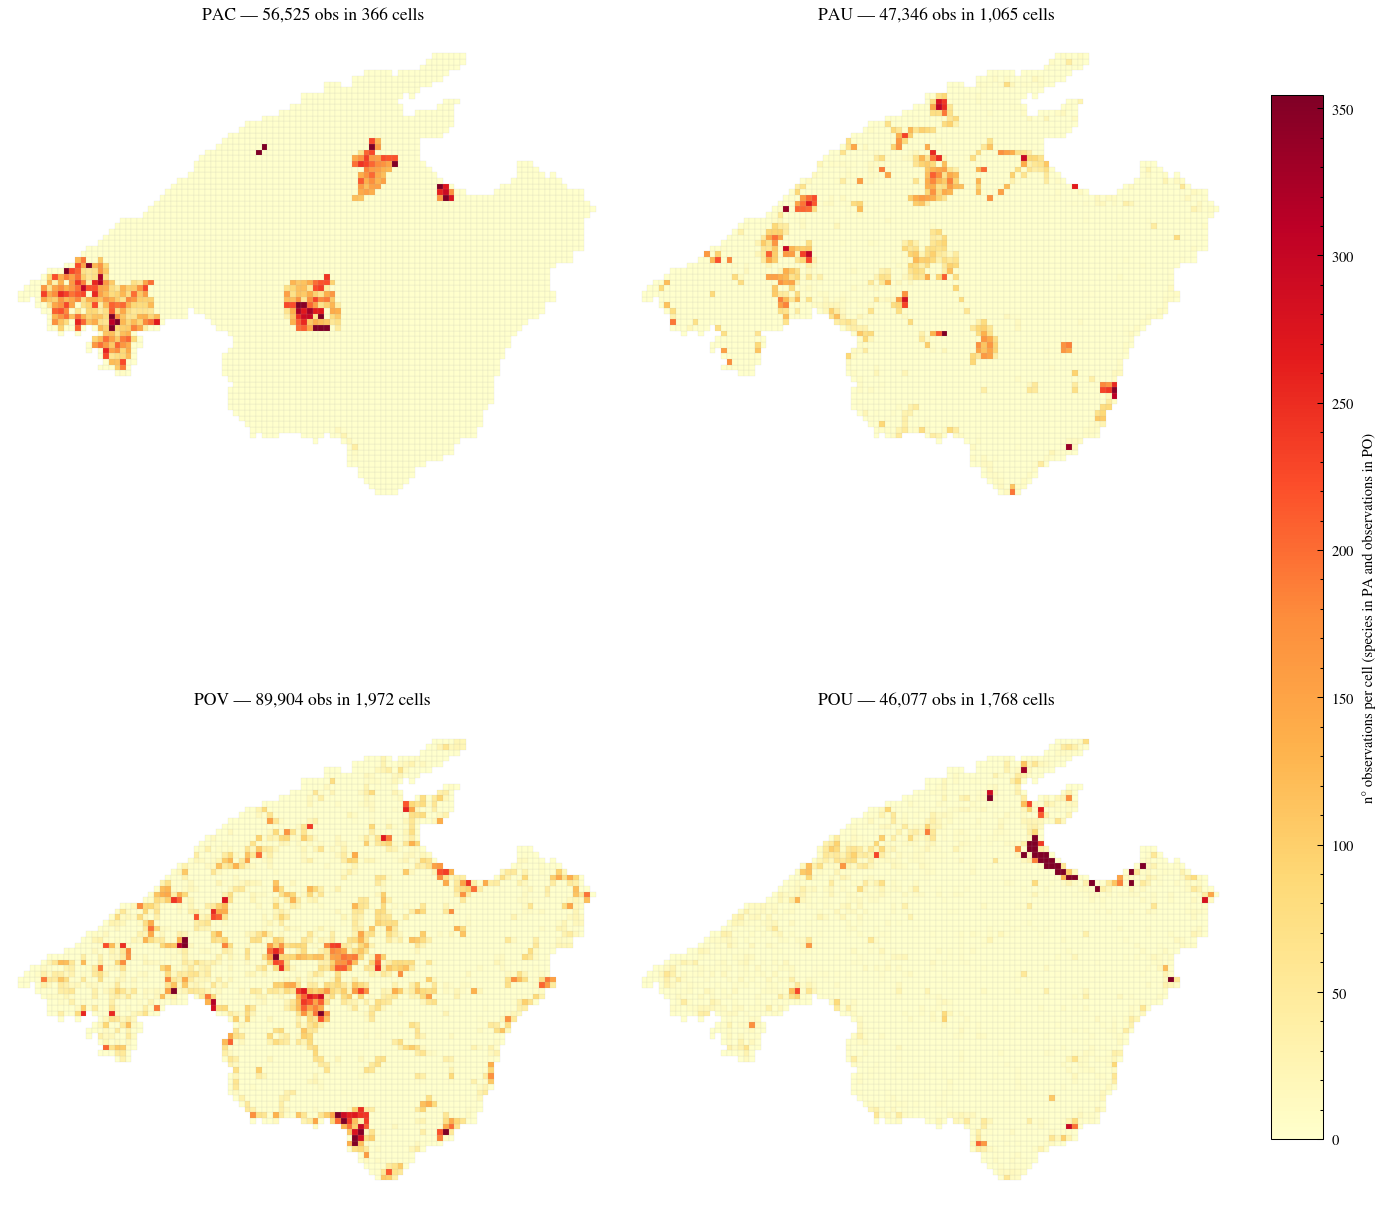
\includegraphics[width=\linewidth]{figures/grid_density_by_source.png}
  \caption{Species density (PA) and observation density (PO) on the $1\times1$\,km Flora grid, by source channel. Preliminary spatial subset.}
  \label{fig:map}
\end{figure}


\subsection{Environmental predictor data}
\label{sec:predictors}

\paragraph{Fine climate.}
Climate covariates come from the dynamically downscaled 1\,km Balearic dataset of \citet{bahuet2026}, covering present and future conditions.
We extract bioclimatic summaries aligned to occurrence locations (project stack \texttt{Bioclim\_CTL\_B1}--\texttt{B19}).
The local downscaling targets island orography and coastal gradients more faithfully than continental CHELSA/WorldClim cubes alone.

\paragraph{Land use and land cover.}
CORINE land-cover classes are one-hot encoded at extraction locations (see project \texttt{covariables.py}).
% TODO: add SIOSE layers in the public release when extract paths are finalised
SIOSE (Spanish high-resolution land-use) is planned as a complementary modality.

\paragraph{Topography and accessibility.}
Elevation and slope enter the tabular feature set; longitude/latitude in EPSG:25831 provide absolute position.
Additional layers contemplated for release include distance to the sea, distance to urban areas, and soil composition.
% TODO: confirm which distance/soil rasters ship in v1

\paragraph{Taxonomic covariates and embeddings.}
Because taxa are identified and backbone-linked after expert review, MallorcaPlant exposes taxonomy as a first-class modality: hierarchical indicators and/or learned taxonomic embeddings shared across species heads.

\paragraph{Satellite embeddings (non-AlphaEarth).}
We plan to attach satellite-derived embeddings (e.g.\ Sentinel-2 features or foundation models that are not pretrained on GBIF occurrence footprints).
We \textbf{exclude AlphaEarth} and similar GBIF-conditioned representations to avoid circular evaluation when POU itself comes from GBIF.
% TODO: choose and document the exact embedding model + tile size in the code release


\subsection{Spatial units and thinning}
\label{sec:spatial}

PAC/PAU observations are represented as cell centroids plus \texttt{coordinateUncertaintyInMeters} (semidiagonal $\approx 707$\,m for $1$\,km cells; $\approx 354$\,m for $500$\,m cells).
POV/POU are GPS points, optionally aggregated to the same \texttt{UTMCODE1X1} grid (\emph{grouped} mode) so that training grain matches PAC evaluation grain.

Raster extraction samples environmental values at $\sim$100\,m pixels inside PA cells (predict per pixel, aggregate to cell for AUC) and at the GPS location for PO points.
Species catalogue for evaluation: taxa present in at least three PAC cells (pipeline threshold \texttt{MIN\_SPECIES\_LIST\_PAC\_GRIDS}).
Training filters require minimum occurrences per source (documented in the repository README).

Spatial autocorrelation can inflate random-split scores \citep{KOLDASBAYEVA2025103521}.
The release targets leave-one-cluster-out (LOCO) evaluation on PAC geographic clusters; the first baselines below still use a fixed PAC layer pending cluster lock.
% TODO: lock PAC clusters + LOCO folds before camera-ready numbers


\section{MallorcaPlant Benchmark}
\label{sec:benchmark}

\paragraph{Task.}
Multi-species prediction of relative suitability / occurrence probability on environmental features.
Primary protocol: \textbf{train} on PAU, POV, and/or POU (single source or factorial mixes); \textbf{evaluate} mean per-species ROC-AUC on PAC cells.
PAC is never used as training labels in the primary track.

\paragraph{Metrics.}
For each species with sufficient PAC support, compute ROC-AUC treating PAC presence/absence as binary ground truth; report the unweighted mean across species.
Optional stratification by PAC prevalence (rare $<5\%$, medium $5$--$30\%$, common $>30\%$ of PAC cells).

\paragraph{Losses.}
When PAU (PA) enters training, baselines use balanced binary cross-entropy.
When only POV/POU are used, baselines use a deep maximum-entropy style loss (batch softmax over sites), avoiding the treatment of non-observed species as true absences at PO sites.

\paragraph{Fair source comparison.}
Point-mode PO training inflates row counts relative to grid PAU.
Grouped (grid-aggregated) PO matrices are required for mix rankings that claim equal spatial support.


\section{Weak and Strong Baselines}
\label{sec:baselines}

We provide weak tabular baselines and stronger multi-species neural baselines on the same splits.

\paragraph{Weak baselines.}
% TODO: fill Table numbers after re-run; do not invent
GLM or MaxEnt-style models on bioclimatic (+ land-cover) features, trained per source or on pooled tabular rows, evaluated on PAC.

\paragraph{Strong baselines.}
A shared multi-layer perceptron (MLP) with residual blocks predicts all catalogue species from standardised environmental features.
Optional taxonomic embedding branch concatenates hierarchy features.
Optimisation uses AdamW with early stopping on a validation split of training sites.

\paragraph{Preliminary source-mix results.}
On a processed spatial subset (order $10^3$ PAU cells; hundreds of PAC evaluation cells), a factorial mix of $\{0,50,100\}\%$ of each training source (point-mode PO; five epochs) yielded a best mean PAC AUC of approximately \textbf{0.763} for PAU/POV/POU $=100/100/50\%$, versus roughly \textbf{0.62--0.70} when POV was excluded (Table~\ref{tab:mix}).
These figures are \emph{preliminary}, confound grain (point PO vs.\ grid PAU), and must be recomputed under grouped PO and LOCO before claims harden.

\begin{table}[t]
  \centering
  \caption{Preliminary source-mix ranking (point-mode PO training; five epochs). Values from early project runs; TBD under grid-grouped PO + spatial CV.}
  \label{tab:mix}
  \begin{tabular}{clcc}
    \toprule
    Rank & Mix (PAU / POV / POU \%) & Train rows & Mean PAC AUC \\
    \midrule
    1 & $100/100/50$ & 86\,657 & 0.763 \\
    2 & $100/100/100$ & 94\,176 & 0.758 \\
    3 & $0/100/100$ & 93\,111 & 0.757 \\
    \midrule
    low & $100/0/0$ (PAU only) & 1\,065 & 0.664 \\
    low & $50/0/0$ & 532 & 0.622 \\
    \bottomrule
  \end{tabular}
\end{table}

\begin{figure}[t]
  \centering
  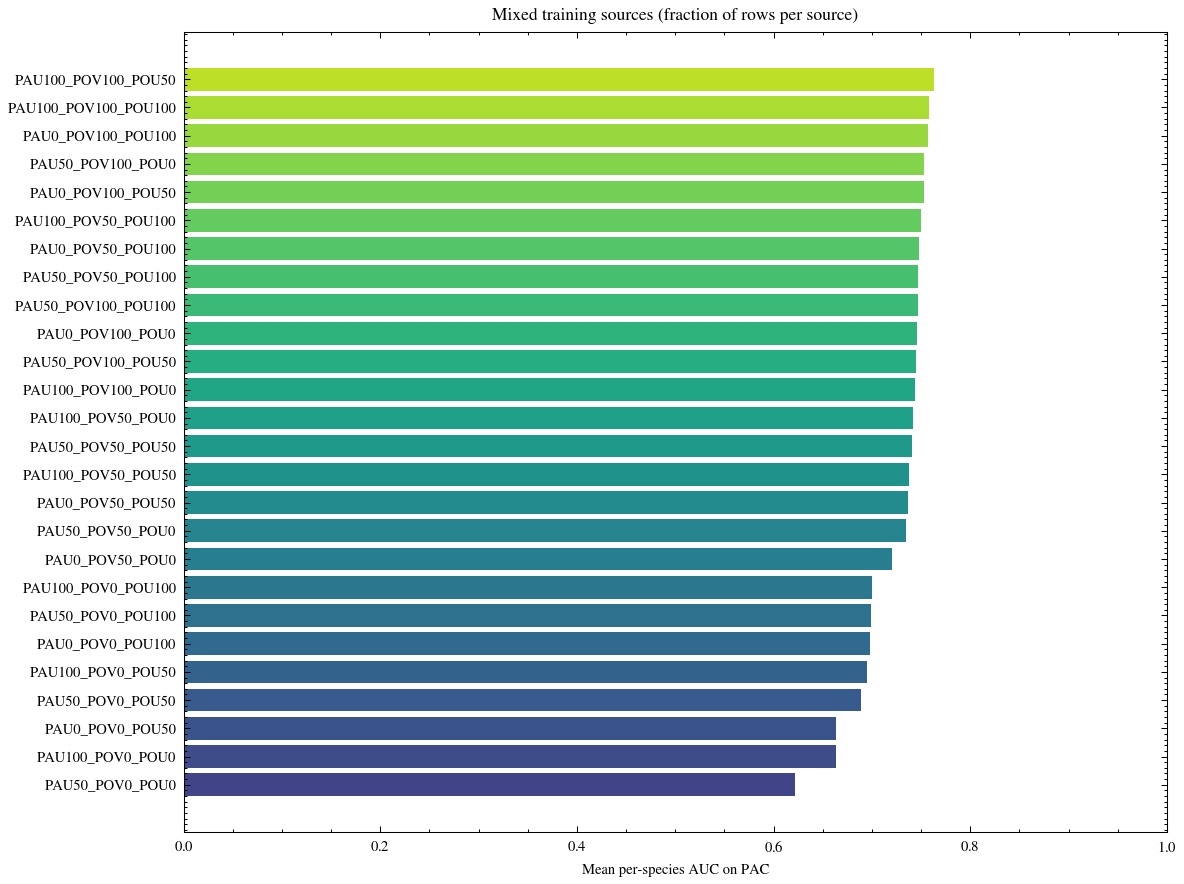
\includegraphics[width=\linewidth]{figures/optimal_model_auc.png}
  \caption{Preliminary factorial mixes of PAU/POV/POU fractions versus mean PAC AUC. Early run; grid-aligned recomputation pending.}
  \label{fig:mix}
\end{figure}

\begin{figure}[t]
  \centering
  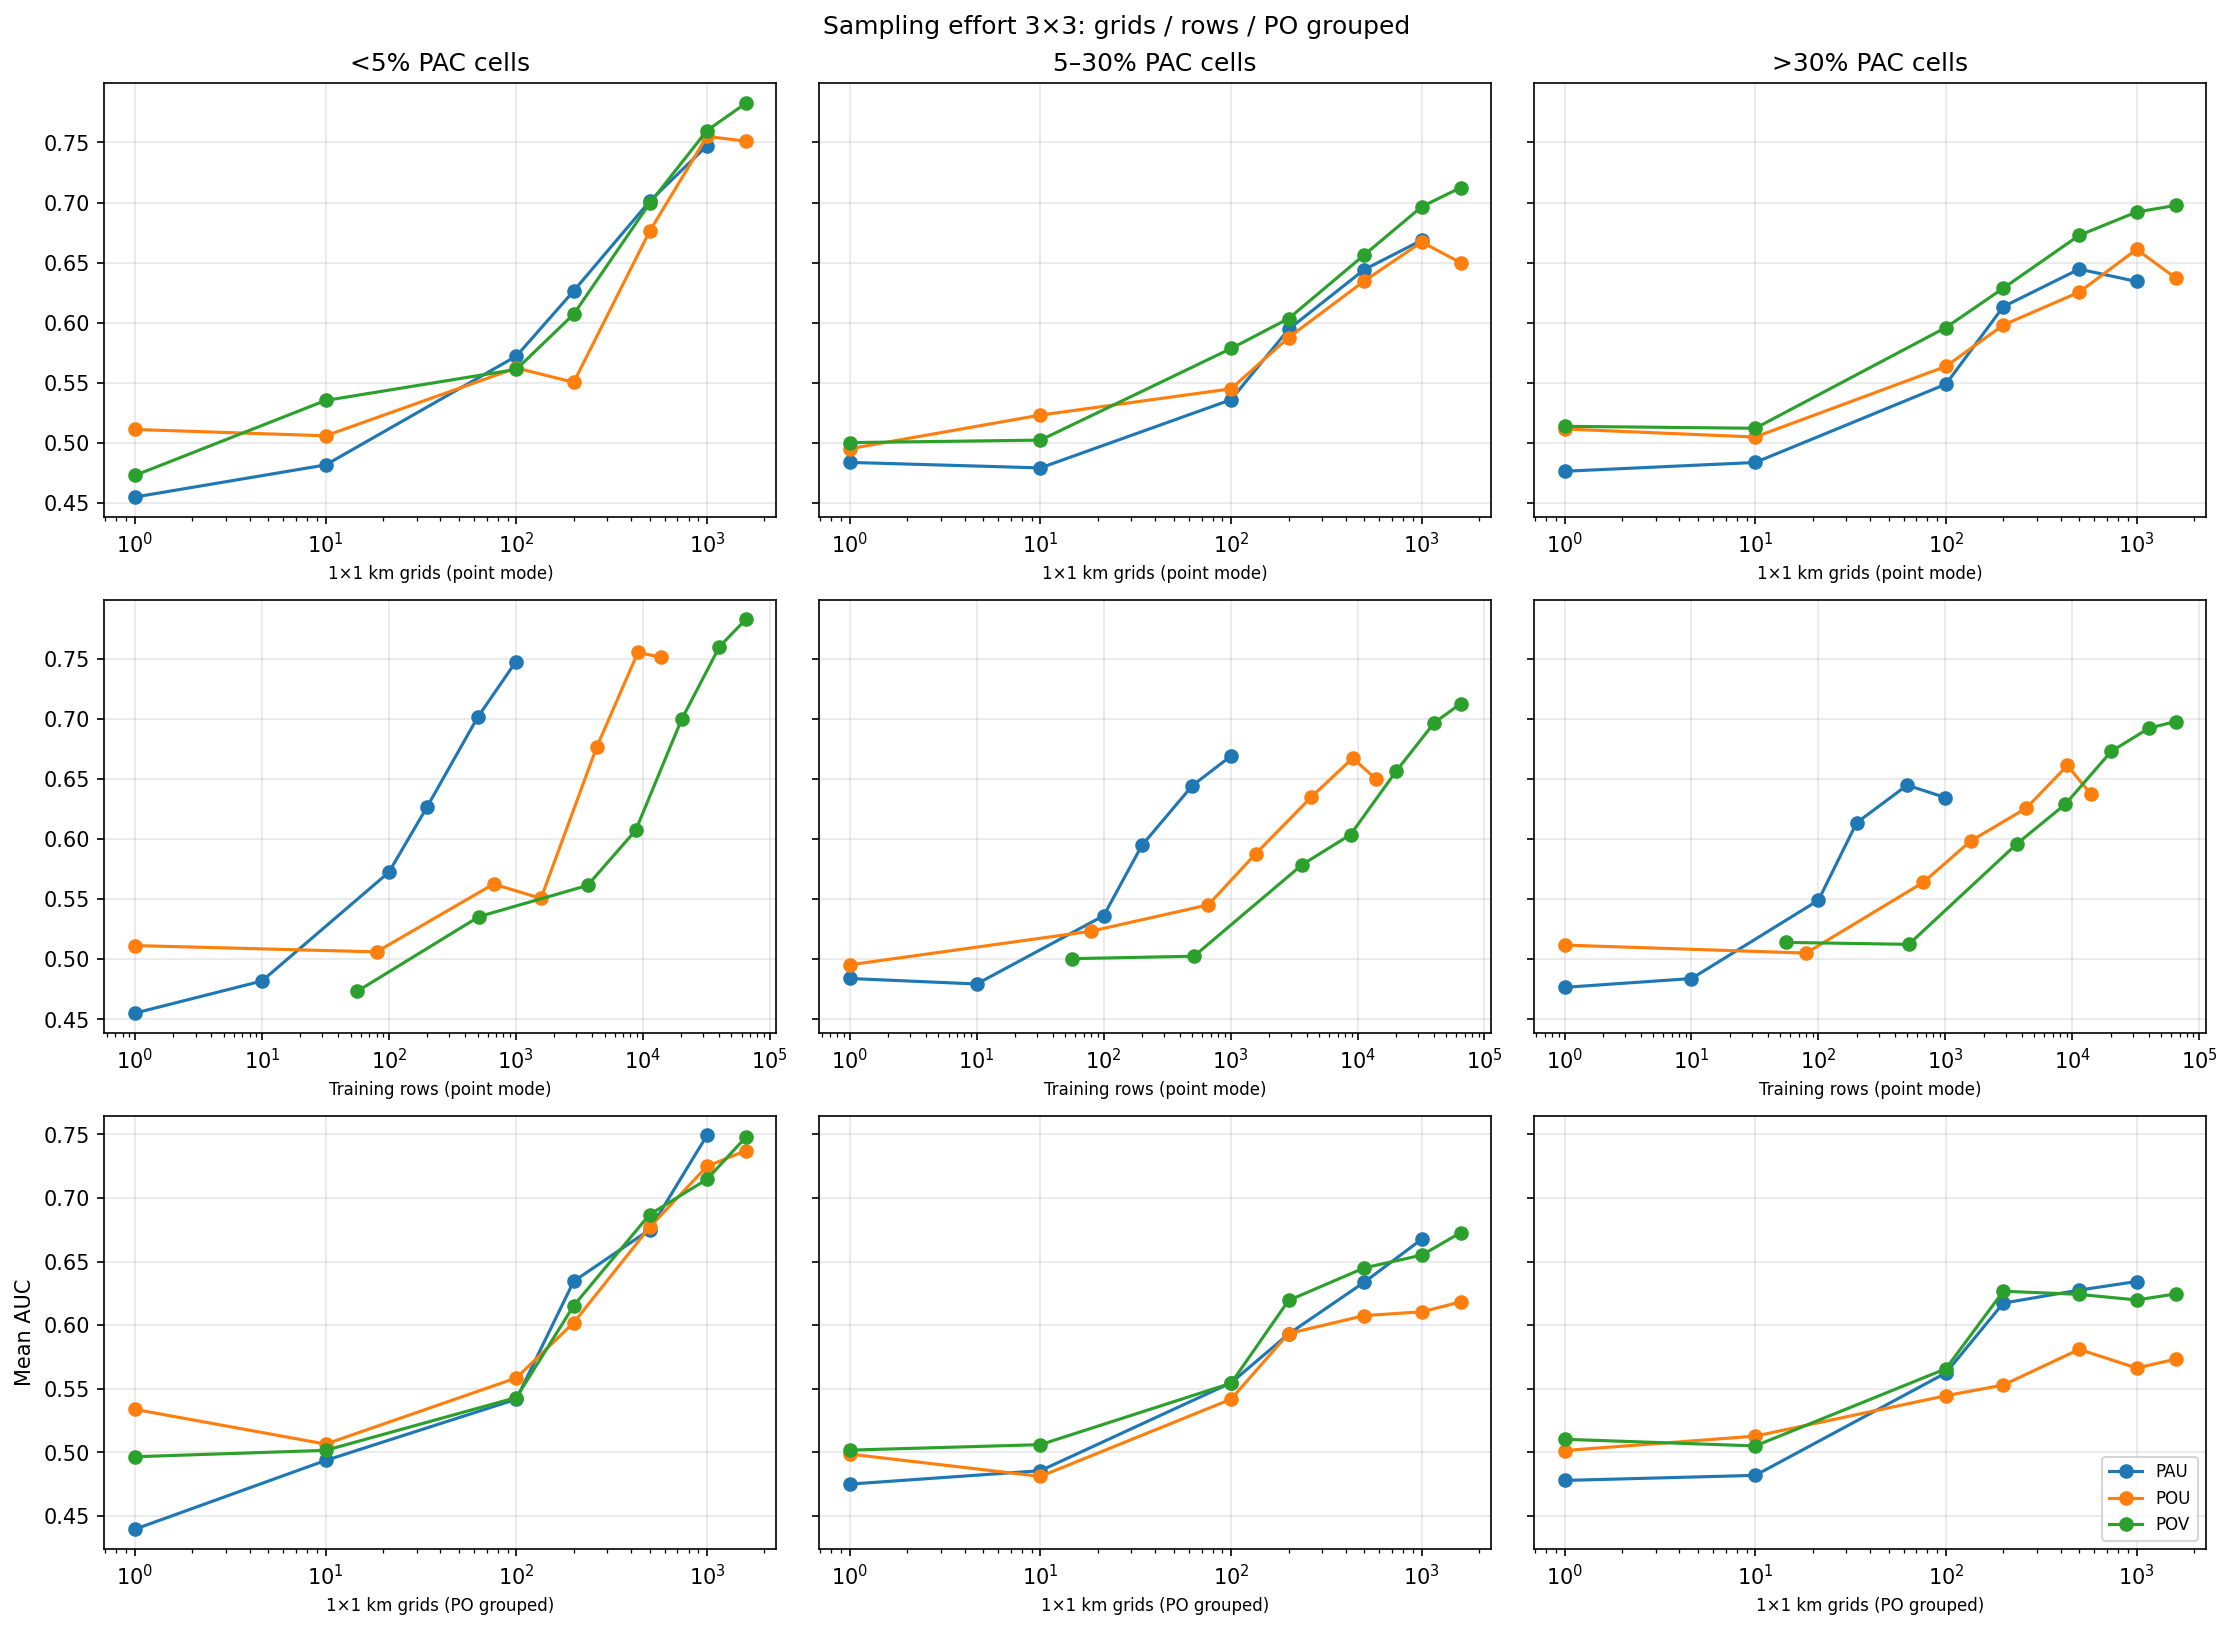
\includegraphics[width=\linewidth]{figures/sampling_effort_auc_by_prevalence.png}
  \caption{Sampling-effort curves: mean PAC AUC versus number of training grids/rows, stratified by PAC prevalence and source (point vs.\ grouped modes in the pipeline). Preliminary spatial subset.}
  \label{fig:effort}
\end{figure}

\paragraph{Modality ablations.}
% TODO: tabular climate-only vs.\ +CORINE vs.\ +taxonomy vs.\ +embeddings once extracts land
Ablations across modalities are part of the release checklist: climate-only, climate+land cover, +taxonomy, +satellite embeddings.


\section{Conclusion}
\label{sec:conclusion}

MallorcaPlant packages four decades of Mallorcan plant surveys into an SDM-ready resource with explicit PAC/PAU/POV/POU semantics, expert-validated PO, and one-by-one taxonomic curation---including names that aggregators miss or reject.
Hidden PA-as-PO encodings and undated atlas tables elsewhere make sampling coverage hard to recover; author-informed labels on Mallorca make that structure usable.
Predictors combine downscaled Balearic climate \citep{bahuet2026}, land use, topography, taxonomic features, and embeddings that avoid GBIF-pretrained AlphaEarth circularity.
Preliminary baselines suggest validated POV carries strong transfer signal to PAC; final rankings require full coverage, grouped PO, and spatial block CV.
Code and processed matrices will accompany the public release; raw heavy rasters remain on institutional storage.


\section*{Acknowledgments and Disclosure of Funding}
We thank the Flora and Biodibal data authors and curators who clarified survey completeness, validation status, and taxonomic decisions.
% TODO: funding statements, conflict of interest, full acknowledgements


\begin{thebibliography}{99}

\bibitem[Atsumi et~al.(2024)]{atsumi2024boosting}
K.~Atsumi et~al.
\newblock Boosting biodiversity monitoring using smartphone-driven, rapidly accumulating community-sourced data.
\newblock \emph{eLife}, 13:RP93694, 2024.

\bibitem[Bahuet-Bourret et~al.(2026)]{bahuet2026}
Y.~Bahuet-Bourret, T.~Cancellario, D.~Arg\"ueso, E.~Arboleda, M.~\`A.~Conesa, J.~M.~Escalona, et~al., and M.~Capa.
\newblock Dynamically downscaled 1-km climate dataset for the Balearic Islands under present and future conditions.
\newblock \emph{Scientific Data}, 2026.

\bibitem[Barbet-Massin et~al.(2012)]{barbet2012selecting}
M.~Barbet-Massin, F.~Jiguet, C.~H.~Albert, and W.~Thuiller.
\newblock Selecting pseudo-absences for species distribution models: How, where and how many?
\newblock \emph{Methods in Ecology and Evolution}, 3(2):327--338, 2012.

\bibitem[Chefaoui and Lobo(2008)]{chefaoui2008assessing}
R.~M.~Chefaoui and J.~M.~Lobo.
\newblock Assessing the effects of pseudo-absences on predictive distribution model performance.
\newblock \emph{Ecological Modelling}, 210(4):478--486, 2008.

\bibitem[Fletcher et~al.(2019)]{fletcher2019practical}
R.~J.~Fletcher~Jr et~al.
\newblock A practical guide for combining data to model species distributions.
\newblock \emph{Ecology}, 100(6):e02710, 2019.

\bibitem[Grattarola et~al.(2023)]{Grattarola2023}
F.~Grattarola, D.~E.~Bowler, and P.~Keil.
\newblock Integrating presence-only and presence--absence data to model changes in species geographic ranges: An example in the Neotropics.
\newblock \emph{Journal of Biogeography}, 50(9):1561--1575, 2023.

\bibitem[Isaac et~al.(2020)]{isaac2020data}
N.~J.~B.~Isaac et~al.
\newblock Data integration for large-scale models of species distributions.
\newblock \emph{Trends in Ecology \& Evolution}, 35(1):56--67, 2020.

\bibitem[Jeliazkov et~al.(2022)]{jeliazkov2022rare}
A.~Jeliazkov et~al.
\newblock Sampling and modelling rare species: Conceptual guidelines for the neglected majority.
\newblock \emph{Global Change Biology}, 28(12):3754--3777, 2022.

\bibitem[Koldasbayeva and Zaytsev(2025)]{KOLDASBAYEVA2025103521}
D.~Koldasbayeva and A.~Zaytsev.
\newblock Foundation for unbiased cross-validation of spatio-temporal models for Species Distribution Modeling.
\newblock \emph{Ecological Informatics}, 92:103521, 2025.

\bibitem[Lobo et~al.(2010)]{lobo2010uncertain}
J.~M.~Lobo, A.~Jim\'enez-Valverde, and J.~Hortal.
\newblock The uncertain nature of absences and their importance in species distribution modelling.
\newblock \emph{Ecography}, 33(1):103--114, 2010.

\bibitem[Phillips et~al.(2009)]{phillips2009sample}
S.~J.~Phillips et~al.
\newblock Sample selection bias and presence-only distribution models: implications for background and pseudo-absence data.
\newblock \emph{Ecological Applications}, 19(1):181--197, 2009.

\bibitem[Picek et~al.(2024)]{geoplant2024}
L.~Picek, C.~Botella, M.~Servajean, C.~Leblanc, R.~Palard, T.~Larcher, B.~Deneu, D.~Marcos, P.~Bonnet, and A.~Joly.
\newblock GeoPlant: Spatial Plant Species Prediction Dataset.
\newblock In \emph{NeurIPS 2024 Datasets and Benchmarks Track}, 2024.
\newblock arXiv:2408.13928.

\bibitem[Rahimi and Jung(2025)]{insects16080769}
E.~Rahimi and C.~Jung.
\newblock Investigating the spatial biases and temporal trends in insect pollinator occurrence data on GBIF.
\newblock \emph{Insects}, 16(8):769, 2025.

\bibitem[Ruiz-Valero et~al.(2025)]{Datafusion2025}
\'A.~Ruiz-Valero, J.~F.~Pere\~na-Ortiz, and \'A.~E.~Salvo-Tierra.
\newblock Data fusion and integrated species distribution models for three endangered ferns in a Mediterranean biodiversity hotspot.
\newblock \emph{Frontiers in Plant Science}, 16:1650159, 2025.

\bibitem[Simmonds et~al.(2020)]{simmonds2020more}
E.~G.~Simmonds et~al.
\newblock Is more data always better? A simulation study of benefits and limitations of integrated distribution models.
\newblock \emph{Ecography}, 43(10):1413--1422, 2020.

\end{thebibliography}


\appendix

\section{Excluded taxonomic orders and families}
\label{app:taxfilters}

Records assigned to the following \textbf{orders} were removed (bryophytes, macroalgae, and related non-target groups):
Bryales, Bryopsidales, Ceramiales, Cladophorales, Corallinales, Dasycladales, Dicranales, Fossombroniales, Funariales, Hypnales, Jungermanniales, Marchantiales, Nemaliales, Pelliales, Peyssonneliales, Porellales, Pottiales, Scouleriales, and Siphonocladales.

Records assigned to the following \textbf{families} were additionally excluded (including marine angiosperms and other non-target aquatic/algal groups):
Posidoniaceae, Potamogetonaceae, Ulvaceae, Phyllophoraceae, Ceratophyllaceae, Anadyomenaceae, Zosteraceae, Ruppiaceae, Bonnemaisoniaceae, Cymodoceaceae, and Hydrocharitaceae.

These filters retain terrestrial vascular plants relevant to the MallorcaPlant ecological analyses.


\section{NeurIPS Datasets \& Benchmarks checklist (draft)}
\label{app:checklist}

Answers below are honest for this draft stage; update at submission.

\begin{enumerate}
  \item \textbf{Motivation.} Yes --- precision multi-source SDM dataset with PAC/PAU/POV/POU semantics and long-term local surveys.
  \item \textbf{Composition.} Occurrence records + environmental rasters + planned embeddings; documentation in README/code.
  \item \textbf{Collection.} Existing Flora, regional validated PO, GBIF, and local inventories; author contact for PAC/PAU.
  \item \textbf{Preprocessing.} Case-by-case taxonomic backbone matching; marine/non-target filters (Appendix~\ref{app:taxfilters}); uncertainty thresholds.
  \item \textbf{Uses.} SDM benchmarking; not a substitute for IUCN assessment or operational conservation maps.
  \item \textbf{Distribution.} Code/matrices via project repository; heavy rasters via institutional NAS --- \emph{TODO public DOI}.
  \item \textbf{Maintenance.} Product Lead: I.~Cort\'es-Fern\'andez; collaborator P.~Ubilla (INRIA).
  \item \textbf{Ethics / privacy.} Biodiversity coordinates may be sensitive for rare taxa --- \emph{TODO} coarsening policy for public PO of threatened species.
\end{enumerate}


\section*{Notes for coauthors (not for submission)}
\begin{itemize}
  \item \texttt{main-2.tex} holds the earlier IDM/methods scratchpad (paper~2 material).
  \item Confirm author list, embedding model, SIOSE inclusion, and Diego sign-off before freeze.
  \item Re-lock Table~\ref{tab:mix} and Figures~\ref{fig:mix}--\ref{fig:effort} after grouped-PO + full extract.
\end{itemize}

\end{document}
